\documentclass[oneside,a4paper,11pt,explicit]{book}
\usepackage[utf8]{inputenc}
\usepackage{icecream}
\usepackage[english]{babel}
\addto\captionsenglish{\renewcommand{\chaptername}{}}
\usepackage[accsupp]{axessibility}  % improves PDF readability for those with disabilities.
\usepackage[hidelinks,colorlinks = true,urlcolor  = blue]{hyperref}
\usepackage{lipsum}
\usepackage{listings}
\usepackage{minitoc}
\addto{\captionsenglish}{% Making babel aware of special titles
	\renewcommand{\mtctitle}{Quick Links To Sections}
}

\title{I.C.E.C.R.E.A.M. Tutorials}
\subtitle{\small Observing Earth from Above (Env 329) - Fall 2023  \\
	\small Schmid College of Science and Technology Chapman University}
\date{\today}

%% DOCUMENT
\begin{document}
	
\dominitoc

\setcounter{chapter}{3} %Insert (Tutorial Number-1) Here; example for tutorial 4, enter 3

\chapter{Adding Elements To Maps} %Enter Tutorial Name Here

\vspace{-2em}

\minitoc

\hrule

\vspace{1em}

\kulbox{{\textbf{\underline{Objectives:}}}

\begin{enumerate}
	\item Learn the map making features in QGIS.
	\item Introduce basic map elements.
	\item Create a NASA worthy map of surface temperatures from Death Valley National Park.
\end{enumerate}
}

\vspace{1 em}

\textbf{\underline{Motivation For Today's Tutorial : NASA Press Releases}}

\vspace{1 em}

{\centering

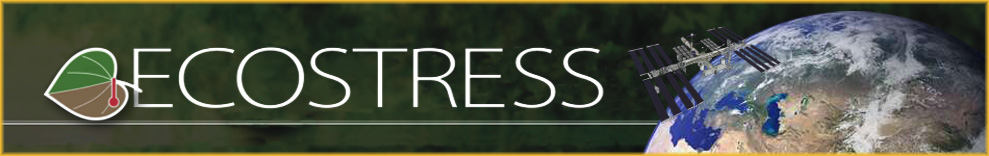
\includegraphics[width=\textwidth]{ecostress_banner.jpg}}

\vspace{1 em}

The idea of this course is to change the way we approach climate disaster analyses and immerse you in the process of science communication. Today we are going to create a publish worthy map of the Death Valley National Park surface temperature experiment we ran in last class. Today's tutorial will provide you with the basic working knowledge to create beautiful and informative maps. Later in the course you will use these skills to analyze current climate disasters and publish your maps through NASA's Jet Propulsion Lab.

\vspace{1 em}

\hrule

\clearpage

\vspace*{.25 em}

\section{Create A Base Map}

{\centering
	
	\includegraphics[width=\textwidth]{Basemap.png}}

1. Create a new project (\textit{Project} $\rightarrow$ \textit{New})

2. Add the ESRI National Geographic Basemap by either:
\begin{itemize}
	\item Using the \textit{XYZ Tiles} function in the \textit{Browser} window
	\item Using the *HCMGIS* Menu (*HCMGIS* $\rightarrow$ *Basemaps* $\rightarrow$ *ESRI National Geographic*)
\end{itemize}

3. Zoom in to California.

\vspace{.25em}

{\centering
	
	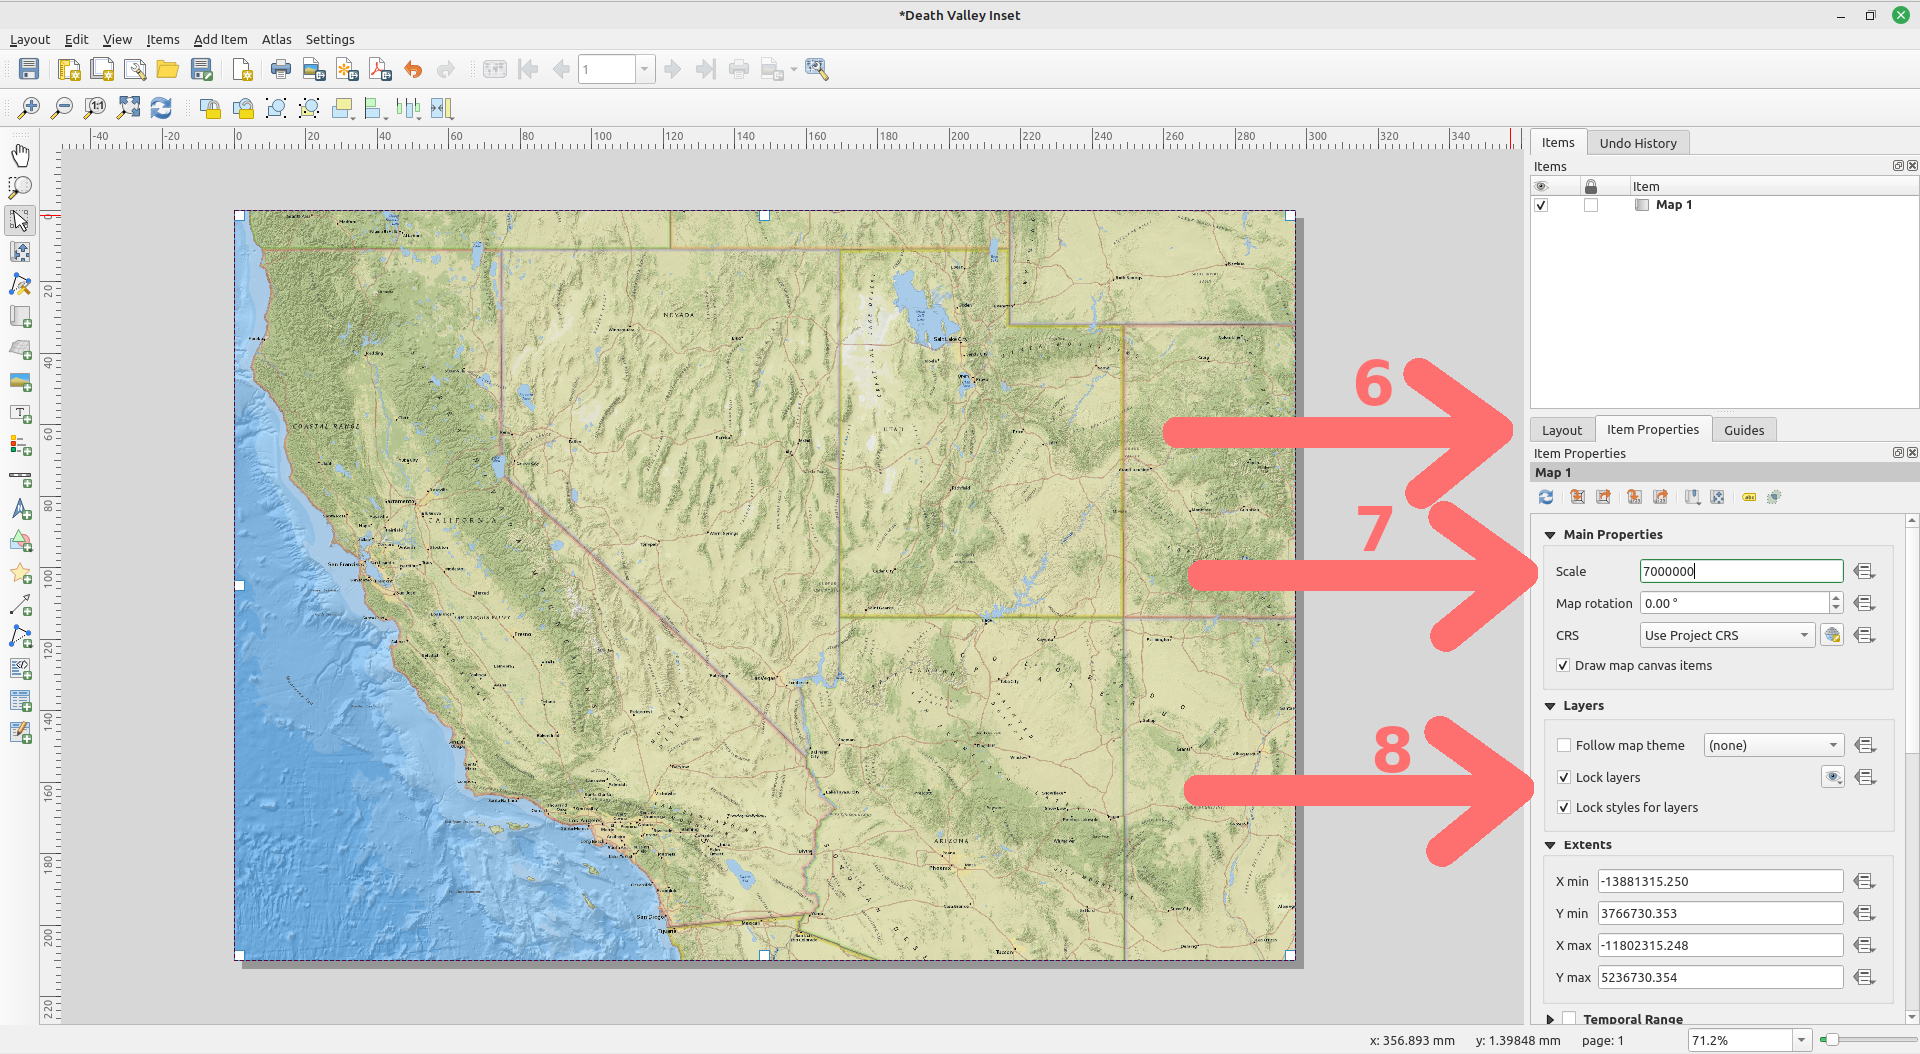
\includegraphics[width=\textwidth]{InsetItem.png}}

\clearpage

\vspace*{3.25 em}

4. Start a new print layout by going to the \textit{Project} menu, then select \textit{New Print Layout}. Enter whatever name you would like. I went with \textit{Death Valley Inset}.

5. Now select the menu \textit{Add Item}, then \textit{Add Map}. Start at one corner of the white rectangle window and drag to the opposite diagonal corner to set the map space. You will see that the rectangle window will be rendered with the map from the main QGIS canvas.

6. Click on the \textit{Item Properties} tab.
7. Adjust the \textit{Scale}, which is the zoom level, to 7000000 and hit enter.
8. Check both \textit{Lock layers} and \textit{Lock layer styles} boxes. This will ensure that if we turn off some layers or change their styles, this view will not change.


\section{Add An Inset}

\subsection{Importing Our ECOSTRESS Death Valley Layer From The Previous Tutorial}

\vfill

\hrule

\vspace{2em}

\textbf{Recommended Citation:} Forsythe, J.D., G.R. Goldsmith, and J.B. Fisher. 2023. Observing Earth from Above Tutorials. Chapman University. \url{https://jeremydforsythe.github.io/icecream-tutorials/}

\vspace{1em}

This work is supported by funding from NASA ECOSTRESS Mission Grant \#80NSSC23K0309 (I.C.E. C.R.E.A.M.: Integrating Communication of ECOSTRESS Into Community Research, Education, Applications, and Media).

\end{document}
